% !TeX root = ../dokumentation.tex

\addchap{\langanhang}

\addsec{Projektplan (Gantt-Chart)}

\begin{landscape}
  \begin{figure}[htbp]
    \centering
    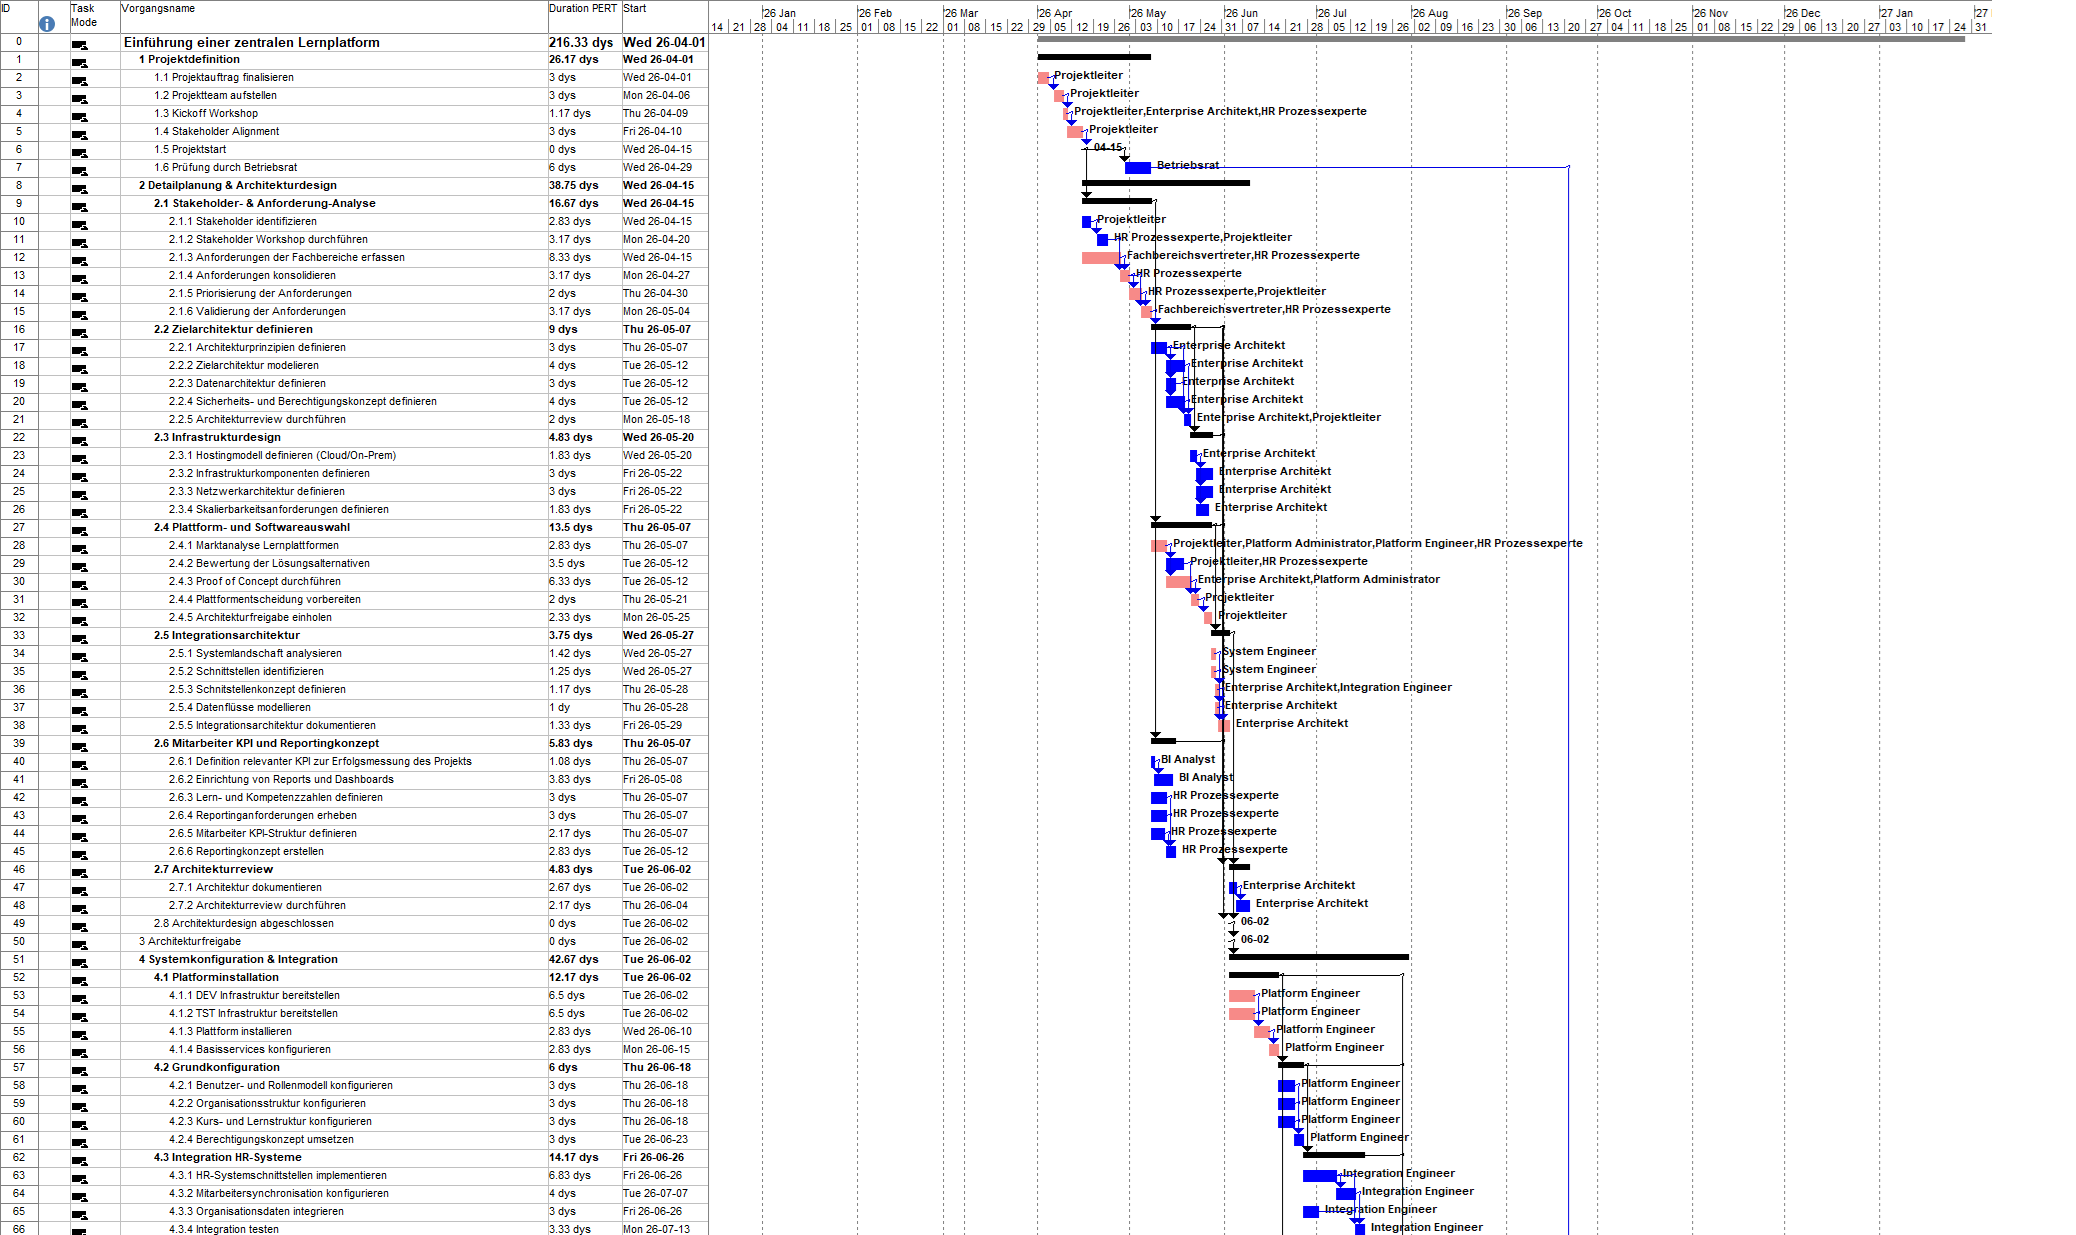
\includegraphics[width=\linewidth]{images/pm26_total_r1_c1_processed_by_imagy.png}
    \caption{Gantt-Chart: Einführung zentrale Lernplattform (Teil 1)}
    \label{fig:gantt-1}
  \end{figure}
  \clearpage
  \begin{figure}[htbp]
    \centering
    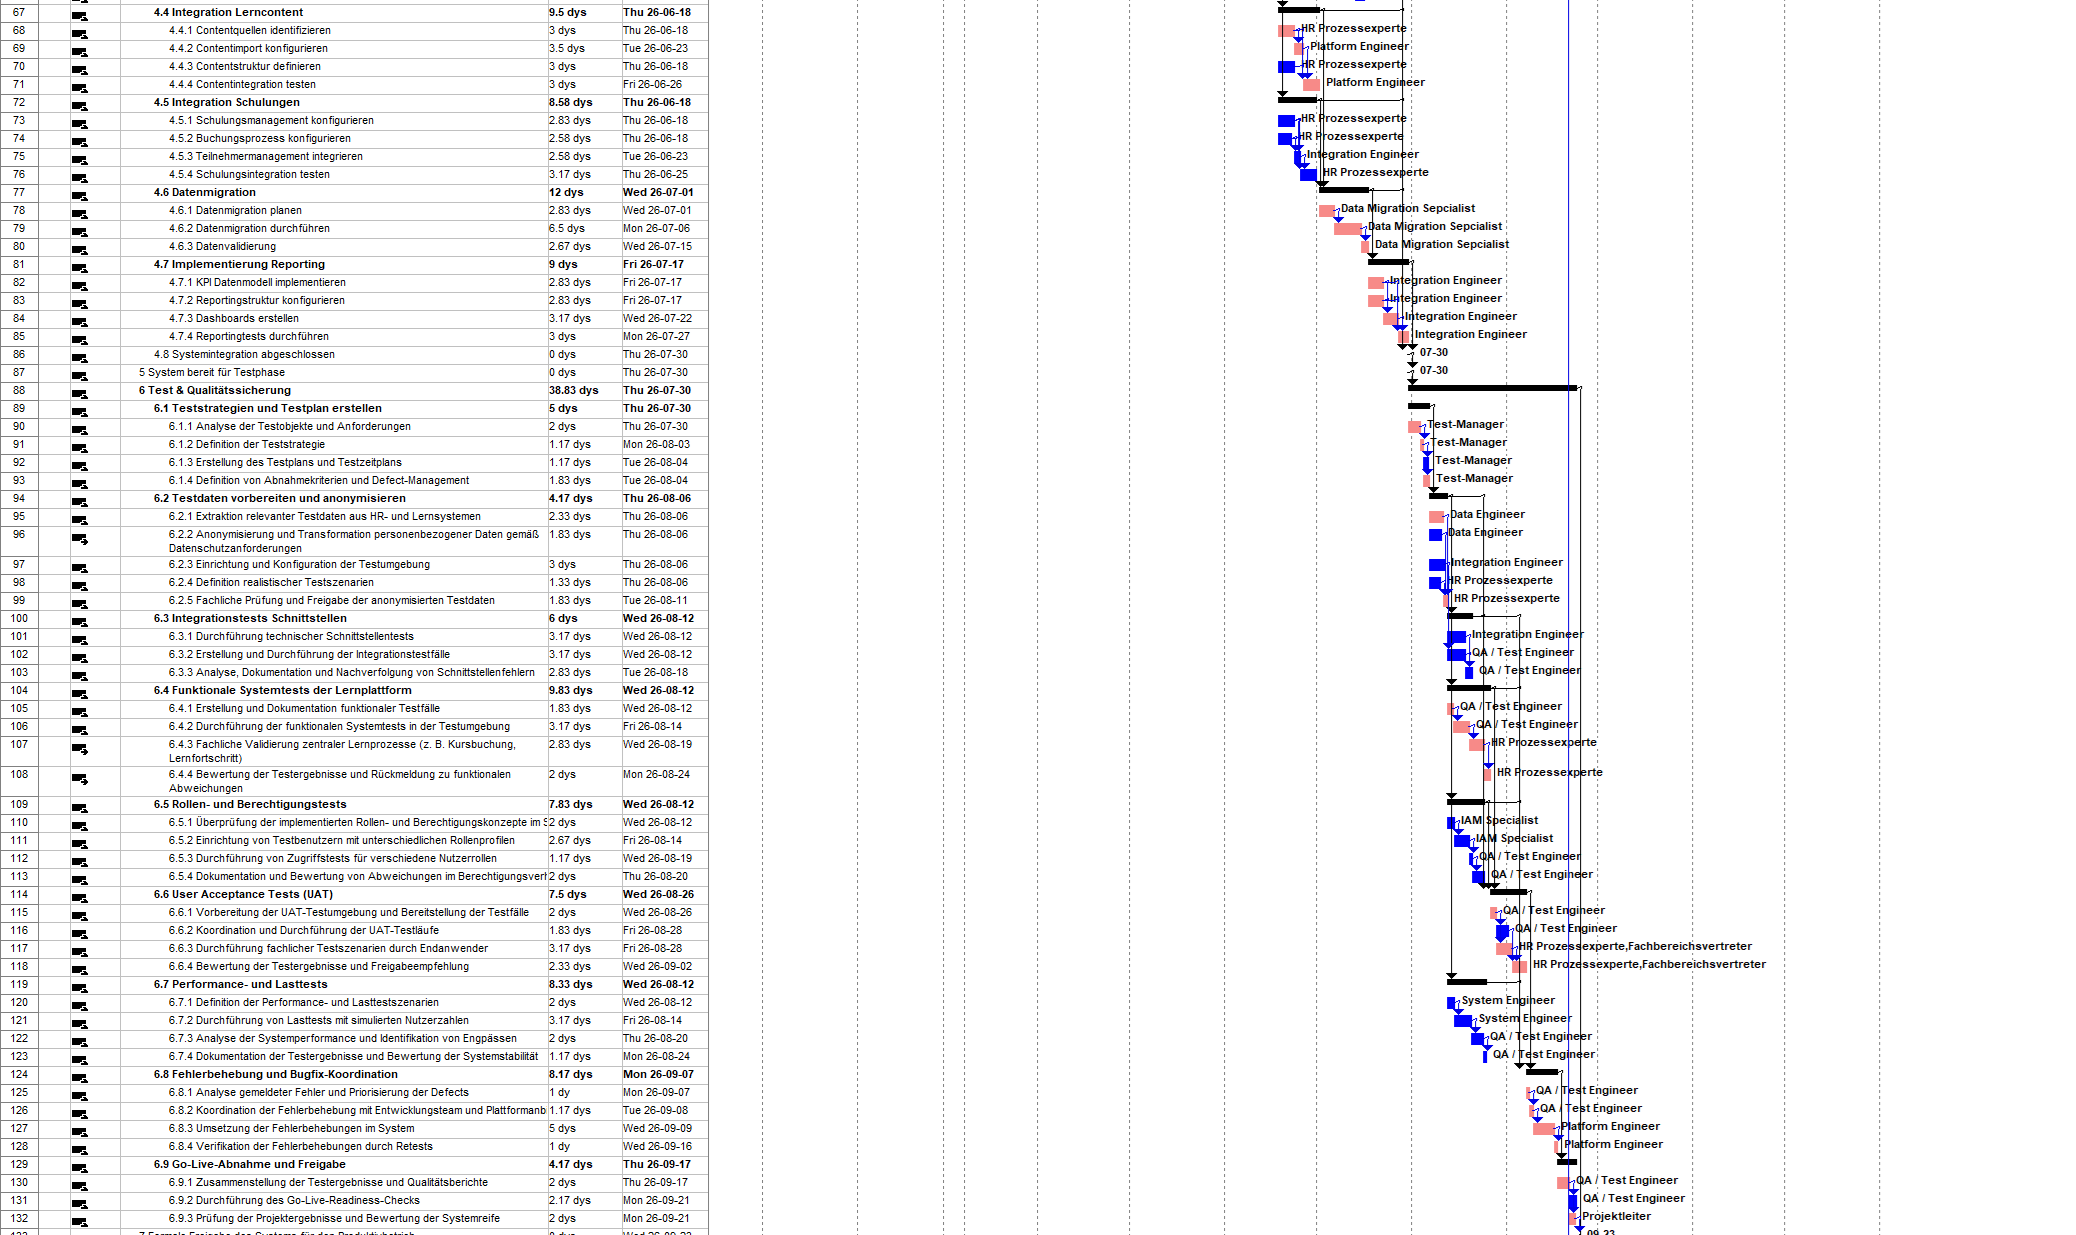
\includegraphics[width=\linewidth]{images/pm26_total_r2_c1_processed_by_imagy.png}
    \caption{Gantt-Chart: Einführung zentrale Lernplattform (Teil 2)}
    \label{fig:gantt-2}
  \end{figure}
  \clearpage
  \begin{figure}[htbp]
    \centering
    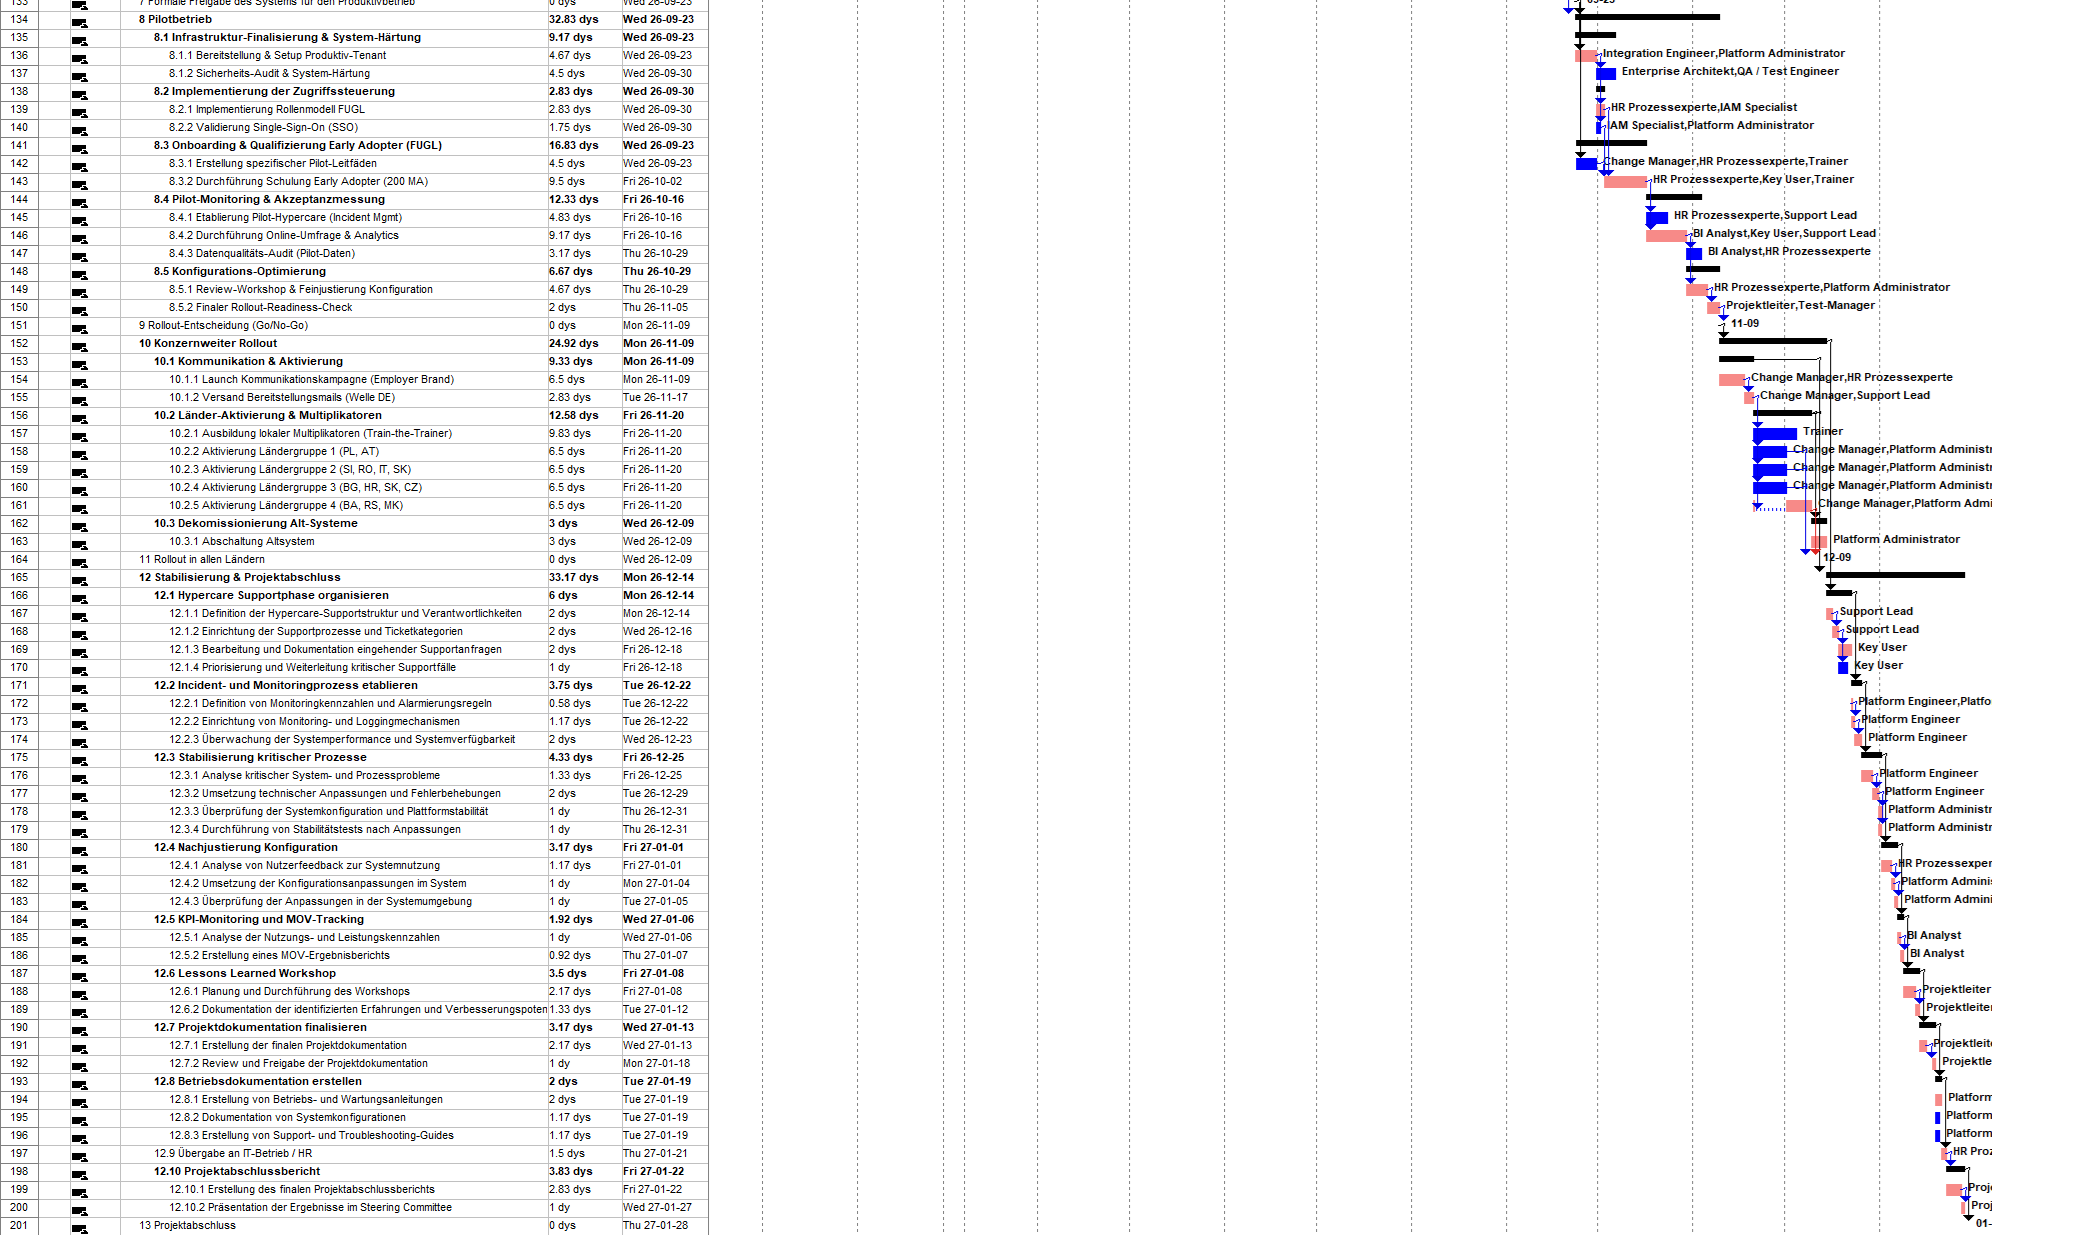
\includegraphics[width=\linewidth]{images/pm26_total_r3_c1_processed_by_imagy.png}
    \caption{Gantt-Chart: Einführung zentrale Lernplattform (Teil 3)}
    \label{fig:gantt-3}
  \end{figure}
\end{landscape}

\addsec{Risikoregister}

\begin{landscape}
  \begin{figure}[htbp]
    \centering
    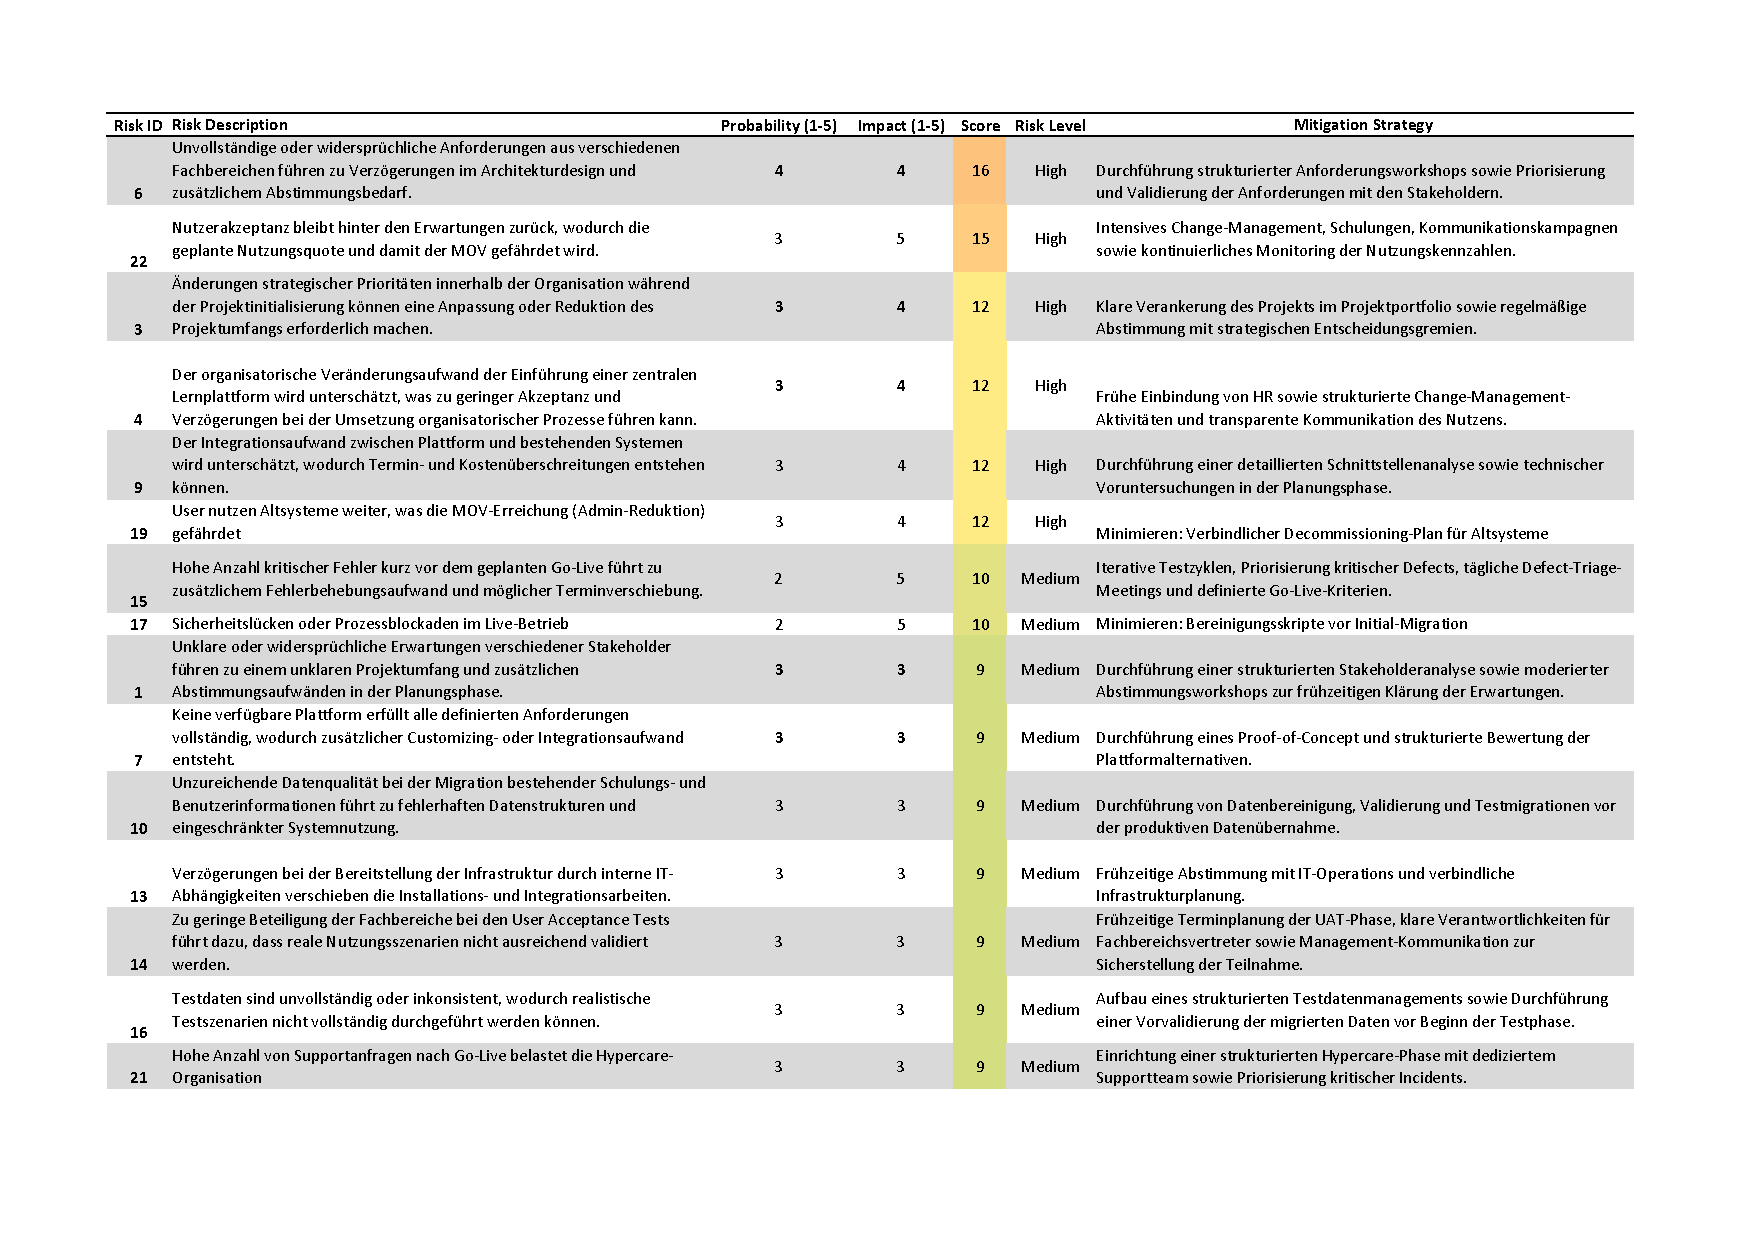
\includegraphics[width=\linewidth]{images/RiskRegister.pdf}
    \caption{Risikoregister: Einführung zentrale Lernplattform}
    \label{fig:risikoregister}
  \end{figure}
\end{landscape}

\addsec{Microsoft Project Makros}

Die folgenden VBA-Makros wurden speziell f\"ur dieses Projekt eigenst\"andig entwickelt,
um PERT-Berechnungen und die Auswertung des kritischen Pfads in Microsoft Project zu
unterst\"utzen.

\begin{lstlisting}[caption={VBA-Makro \texttt{PERTCalculation} fuer Microsoft Project},label={lst:pertcalculation}]
Sub PERTCalculation()

'Declare variable
Dim myTask As Task

'Loop all tasks to update duration
For Each myTask In ActiveProject.Tasks

    If Not (myTask Is Nothing) And Not myTask.Summary And Not myTask.Milestone Then
        
        'Optional: nur wenn alle drei Werte gesetzt sind
        If myTask.Duration1 > 0 And myTask.Duration2 > 0 And myTask.Duration3 > 0 Then
        
            'PERT formula
            myTask.Duration = (myTask.Duration1 + 4 * myTask.Duration2 + myTask.Duration3) / 6
        
        End If
        
    End If

Next myTask

End Sub
\end{lstlisting}

\begin{lstlisting}[caption={VBA-Makro \texttt{PERTCriticalPathFullStats} fuer Microsoft Project},label={lst:pertcriticalpathfullstats}]
Option Explicit

Sub PERTCriticalPathFullStats()

    Dim t As Task
    
    Dim totalMeanDays As Double
    Dim totalVariance As Double
    Dim totalStdDevDays As Double
    
    Dim criticalTasks As Long
    
    Dim targetDays As Double
    Dim zValue As Double
    Dim probability As Double
    
    Dim inputValue As String
    Dim minutesPerDay As Double
    
    minutesPerDay = ActiveProject.HoursPerDay * 60
    
    totalMeanDays = 0
    totalVariance = 0
    totalStdDevDays = 0
    criticalTasks = 0

    For Each t In ActiveProject.Tasks
    
        If Not t Is Nothing Then
            If Not t.Summary And Not t.Milestone Then
                If t.Critical Then
                    
                    ' Duration in MS Project is stored in minutes -> convert to days
                    totalMeanDays = totalMeanDays + (t.Duration / minutesPerDay)
                    
                    ' Number2 contains variance in days^2
                    If IsNumeric(t.Number2) Then
                        totalVariance = totalVariance + t.Number2
                    End If
                    
                    criticalTasks = criticalTasks + 1
                End If
            End If
        End If
        
    Next t

    totalStdDevDays = Sqr(totalVariance)

    inputValue = InputBox( _
        Prompt:="Bitte Zieldauer in Tagen (in Tagen) eingeben, fuer die Z-Value und Probability berechnet werden sollen:", _
        Title:="PERT Z-Value und Probability" _
    )
    
    If inputValue = "" Then
        MsgBox "Abgebrochen.", vbInformation, "PERT"
        Exit Sub
    End If
    
    If Not IsNumeric(inputValue) Then
        MsgBox "Ungueltige Eingabe. Bitte eine Zahl in Tagen eingeben.", vbExclamation, "PERT"
        Exit Sub
    End If
    
    targetDays = CDbl(inputValue)

    If totalStdDevDays > 0 Then
        zValue = (targetDays - totalMeanDays) / totalStdDevDays
        probability = NormalCDF(zValue)
    Else
        zValue = 0
        
        If targetDays >= totalMeanDays Then
            probability = 1
        Else
            probability = 0
        End If
    End If

    MsgBox _
        "PERT Ergebnisse (Critical Path)" & vbCrLf & vbCrLf & _
        "Anzahl kritischer Vorgaenge: " & criticalTasks & vbCrLf & _
        "Gesamt Mean Duration: " & FormatNumber(totalMeanDays, 2) & " Tage" & vbCrLf & _
        "Gesamt Varianz: " & FormatNumber(totalVariance, 2) & " Tage^2" & vbCrLf & _
        "Projekt Standardabweichung: " & FormatNumber(totalStdDevDays, 2) & " Tage" & vbCrLf & vbCrLf & _
        "Zieldauer: " & FormatNumber(targetDays, 2) & " Tage" & vbCrLf & _
        "Z-Value: " & FormatNumber(zValue, 4) & vbCrLf & _
        "Probability: " & FormatPercent(probability, 2), _
        vbInformation, "PERT Critical Path"

End Sub


Function NormalCDF(z As Double) As Double

    Dim t As Double
    Dim d As Double
    Dim prob As Double
    Dim poly As Double
    
    Const b1 As Double = 0.31938153
    Const b2 As Double = -0.356563782
    Const b3 As Double = 1.781477937
    Const b4 As Double = -1.821255978
    Const b5 As Double = 1.330274429
    Const p As Double = 0.2316419
    Const c As Double = 0.39894228

    If z >= 0 Then
    
        t = 1 / (1 + p * z)
        d = c * Exp(-z * z / 2)
        
        poly = b5
        poly = b4 + t * poly
        poly = b3 + t * poly
        poly = b2 + t * poly
        poly = b1 + t * poly
        
        prob = 1 - d * t * poly
        
    Else
    
        prob = 1 - NormalCDF(-z)
        
    End If
    
    NormalCDF = prob

End Function
\end{lstlisting}
